\section{Part 1}

\subsection{Forward simulation}
Let 
\begin{itemize}
    \item $\gamma$ be the probability of moving from the state of serial processing to the state of parallel processing
    \item $\beta$ be the probability of moving from the state of parallel processing to either one of the two states of serial processing
    \item $\alpha$ be the probability of neuron $N_{i,j}$ attending $S_1$
    \item $\lambda_k$ be the intensity of the poisson distributed random variables, $X_{i,j}$, when attending to stimulus $S_k$  for $k = 0,1$
\end{itemize}
and define the CPD's of the $C_i$'s given $C_{i-1}$ in the shape of a $\Gamma$-matrix:
\begin{align*}
    \Gamma = \begin{pmatrix}
        1- \gamma & 0 & \gamma\\
        0 & 1- \gamma & \gamma\\
        \beta/2 & \beta/2 & 1-\beta
    \end{pmatrix}
\end{align*}

We initialize the $C_i$'s as a vector recursively with probabilities
\begin{align*}
    P(C_0 = 2 )= 1, \quad 
    P(C_i  = d \mid C_{i-1} = c) = \gamma_{c,d} \for i\in \{2,\ldots, T\},
\end{align*}
where $\gamma_{c,d}$ is the matrix entry $\Gamma_{(c+1, d+1)}$. \footnote{the upper left entry in matrix is denoted as $\Gamma_{1,1}$, so we need make the dimensions match} The CPD's of $Z_i$'s are given as
\begin{align*}
    P(Z_{i,j} = 1 \mid C_i = c) = \begin{cases}
        1- \alpha & \tif c = 0\\
        \alpha & \tif c = 1\\
        \frac{1}{2} &\tif c =2
    \end{cases} \for i \in \{1, \ldots, n\}
\end{align*}
and we generate the $Z_{i,j}$'s from a Bernoulli-distribution. Finally, we build the CPD's for each individual $X_{i,j}$ such that

\begin{align*}
    X_{i,j} \mid Z_{i,j} = z \sim Pois( \lambda_0 + (\lambda_1-\lambda_0)z ) \for i,j \in \{1,\ldots T\}\times \{1,\ldots, n\}
\end{align*}

The data structures after data generation are:

\begin{align*}
    C &= [C_1, C_2, \ldots, C_T],\quad     Z = \begin{bmatrix}
        [Z_{11}, Z_{12}, \ldots, Z_{1T}]\\
        [Z_{21}, Z_{22}, \ldots, Z_{2T}]\\
        \vdots\\
        [Z_{n1}, Z_{n2}, \ldots, Z_{nT}]\\
    \end{bmatrix}, \quad X = \begin{bmatrix}
        [X_{11}, X_{12}, \ldots, X_{1T}]\\
        [X_{21}, X_{22}, \ldots, X_{2T}]\\
        \vdots\\
        [X_{n1}, X_{n2}, \ldots, X_{nT}]\\
    \end{bmatrix}
\end{align*}








\subsection{Illustration of implementation}

\begin{figure}
\centering
  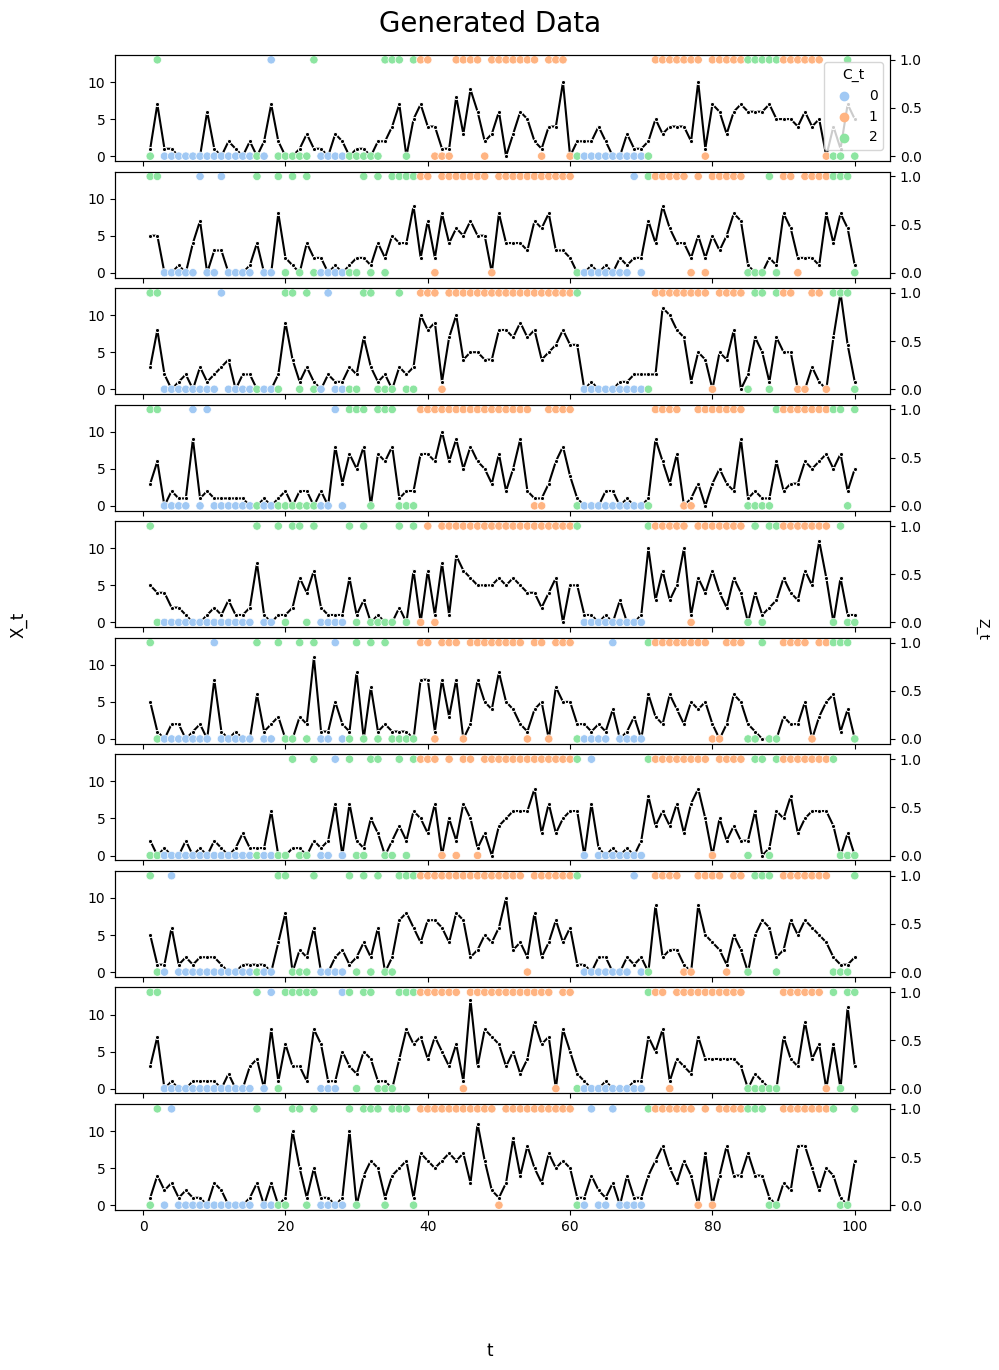
\includegraphics[width=0.9\textwidth]{latex/figures/data_generation_viz.png}
  \caption{Data generation visualization.}
  \label{fig:datagen}
\end{figure}


\subsection{Multinomial Logistic Regression}

The multinomial logistic model models the probability of a response variable $Y$ falling into one of $K=3$ classes, given $p = n \cdot T$ predictor variables $X_1,...,X_p$. The model is of the form 
$$
P(Y=k| X=x) = \frac{\exp(\beta_{k0} + \beta_{k1}x_1 +... + \beta_{kp}x_p)}{1 + \sum_{i=1}^{K-1}\exp(\beta_{l0} + \beta_{l1}x_1 +... + \beta_{lp}x_p)}
$$
For $k = 1,2$, and:
$$
P(Y=K| X=x) = \frac{1}{\exp(\beta_{l0} + \beta_{l1}x_1 +... + \beta_{lp}x_p)}
$$
Multinomial logistic regression estimates coefficients $\beta_{k0},...,\beta_{kp}$. 
We simulate 1000 replicas of the Hidden Markov Model for $T=100$ and $n = 10$. Using this data, we first fit a multi class logistic model predicting $C_{50}$ given all the $X_{i,t}$-variables. Thus the classes $C_{50}$ can fall into are $k=0,1,2$ and the model has $10\cdot 100 = 1000$ predictor variables. The model fit outputs $3 \cdot 10\cdot 100 = 3000$ $\beta$-coefficients, which are difficult to interpret by the mere size (????).
To test the model, we create a new data set again consisting of 1000 replicas of the Hidden Markov Model for $T=100$ and $n = 10$. The accuracy of the logistic model on the new data is 0.664. The larger the training set, the better the accuracy. Increasing the number of simulations to 10000 results in an accuracy of $0.837$. 

We then attempt to predict $C_{50}$ given $X_{1,49},...,X_{10,49},X_{1,50},...,X_{10,50}, X_{1,51},...,X_{10,51}$. This is done,..., conditional independence?. This results in a better accuracy of 0.885. The higher accuracy is due to the overfitting of the previous model.


